\documentclass[10pt,a4paper]{report}
\usepackage[utf8]{inputenc}
\usepackage{ucs}
\usepackage{amsmath}
\usepackage{amsfonts}
\usepackage{amssymb}
\usepackage[english,greek,francais]{babel}
\usepackage{graphicx} 

%Symbole €
\usepackage[LGR,T1]{fontenc}

%Doxygen
\usepackage{a4wide}
\usepackage{makeidx}
\usepackage{fancyhdr}
\usepackage{multicol}
\usepackage{float}
\usepackage{textcomp}
\usepackage{alltt}
\usepackage{doxygen/doxygen}
\renewcommand{\footrulewidth}{0.4pt}

\usepackage{geometry}
\geometry{ hmargin=2.5cm, vmargin=1.8cm }

%page garde
\makeatletter
\def\clap#1{\hbox to 0pt{\hss #1\hss}}%
\def\ligne#1{%
\hbox to \hsize{%
\vbox{\centering #1}}}%
\def\haut#1#2#3{%
\hbox to \hsize{%
\rlap{\vtop{\raggedright #1}}%
\hss
\clap{\vtop{\centering #2}}%
\hss
\llap{\vtop{\raggedleft #3}}}}%
\def\bas#1#2#3{%
\hbox to \hsize{%
\rlap{\vbox{\raggedright #1}}%
\hss
\clap{\vbox{\centering #2}}%
\hss
\llap{\vbox{\raggedleft #3}}}}%
\def\maketitle{%
\thispagestyle{empty}\vbox to \vsize{%
\haut{}{\@blurb}{}
\vfill
\vspace{1cm}
\begin{flushleft}
\usefont{OT1}{ptm}{m}{n}
\huge \@title
\end{flushleft}
\par
\hrule height 4pt
\par
\begin{flushright}
\usefont{OT1}{phv}{m}{n}
\Large \@author
\par
\end{flushright}
\vspace{2.5cm}
\begin{center}
	
\includegraphics[width=7cm]{images/ensib_logo.png}
\end{center}
\vfill
\vfill
\bas{}{\@location, le \@date}{}
}%
\cleardoublepage
}

\def\date#1{\def\@date{#1}}
\def\author#1{\def\@author{#1}}
\def\title#1{\def\@title{#1}}
\def\location#1{\def\@location{#1}}
\def\blurb#1{\def\@blurb{#1}}
\date{\today}
\author{}
\title{}
\location{}
\blurb{}

\makeatother
\blurb{%
ENSI de Bourges\\
Filière Sécurité et Technologies Informatiques\\
\vspace{4cm}
\textbf{Rapport de stage en entreprise}\\[1em]
Maître de stage : Benjamin Venelle\\
Tuteur universitaire : Jérémy Briffaut
}% 
\title{Développement de PIGA-SYSTRANS}
\author{Martin Peres}
\location{Bourges}


\begin{document}
	%intro
	\maketitle
	\begin{abstract}
	\paragraph*{}
		Ce rapport se veut le reflet de mon stage de 1\up{ère} année effectué dans l'entreprise SPIDWARE dirigée par M. Martial Szpieg.\newline
	Vous y trouverez des explications sur l'organisation de l'entreprise et son environnement ainsi qu'un rapport technique sur ma réalisation.
	
	\paragraph*{}
		Je voudrais remercier Martial Szpieg, Jérémy Briffault, Christian Toinard et Jonathan Rouzaud-Cornabas pour leurs conseils et la confiance qu'ils m'ont accordé en me proposant ce stage.
\end{abstract}




	\tableofcontents
	\listoffigures
		
	\chapter*{Introduction}
	\paragraph*{}
		Mon stage de fin de première année s'est déroulé dans la spin-off SPIDWARE initiée par Martial Szpieg et ayant comme but principal de valoriser la recherche effectuée par les chercheurs du projet SDS\footnote{Sécurité et Distribution des Systèmes. Ce projet est porté par l'équipe de chercheurs du Laboratoire d'Informatique Fondamentale d'Orléans (LIFO) basée à l'ENSI de Bourges}.
	
	\paragraph*{}
		Actuellement, le projet SDS	a deux objectifs, remporter le défi sécurité SEC-SI initié par l'ANSSI\footnote{Agence Nationale pour la Sécurité des Systèmes d'Information, anciennement DCSSI: Organisme inter-ministériel officiel visant au conseil et à la validation sur les techniques de sécurité pour l'état et ses administrés} et porté par l'ANR\footnote{Agence Nationale de la Recherche: Ses buts sont de promouvoir la recherche et de la financer} mais aussi la création de l'entreprise SPIDWARE visant à promouvoir la recherche en informatique de l'ENSI de Bourges.
		
	\paragraph*{}
		Le travail actuel se base en grande partie sur la thèse de Jérémy Briffault encadrée par Christian Toinard et qui, après 7 ans de travail a abouti à PIGA\footnote{Policy Interaction Graph Analysis}, un logiciel de détection et prévention d'intrusion. Ce programme a montré sa fiabilité sur le pot de miel\footnote{Serveur ayant l'apparence d'un système non-sécurisé sur lequel des attaquants se connectent. Ce genre de serveur permet d'analyser les types d'attaque informatique actuelles. Malgré les apparences, il se doit d'être extrêmement sécurisé pour ne pas devenir une machine zombie.} de l'école en résistant depuis plus de 3 ans à une moyenne d'une centaine d'attaques par jour. 
	
	\paragraph*{}
		Mon stage à SPIDWARE a duré 3 mois et avait pour objectif la création d'un nouvel outil de sécurité permettant d'amener une gestion des droits à l'intérieur même des applications. Ce firewall applicatif est appelé PIGA-SYSTRANS.\\
		Les applications à protéger sont Firefox, Claws-mail et Open Office. Le choix s'est porté sur celles-ci car elles répondent aux besoins de base de la bureautique.\\
		Au cours de mon stage, j'ai donc travaillé avec les chercheurs en sécurité de l'ENSI de Bourges et notamment avec Jéméry Briffault qui m'a encadré lors de cette réalisation.
	
	\paragraph*{}
		Dans ce rapport, on s'attachera à mieux définir l'environnement dans lequel j'ai travaillé en détaillant un peu plus ce qu'est PIGA, le défi sécurité SEC-SI, SPIDWARE et mon projet, PIGA-SYSTRANS.
		Ensuite, je détaillerai la méthode de travail et de validation de PIGA-SYSTRANS par les chercheurs. Pour finir, je présenterai les évolutions nécessaires pour atteindre une qualité satisfaisante.

\chapter{Environnement de travail}
	\section{PIGA}
		\paragraph*{}
			PIGA est un logiciel permettant de faire de la détection et de la prévention d'intrusion. En d'autres termes, cela permet de savoir si une personne qui n'a normalement pas les droits accéder aux ressources d'un serveur essaye de se les approprier et, si tel est le cas, de l'en empêcher.

		\paragraph*{}
			Le travail sur PIGA a commencé il y a environ 8 ans lors du début de la thèse de Jérémy Briffault, encadrée par Christian Toinard. Le projet a progressivement muri au point de défaire chaque jour plus d'une centaine d'attaque sur le pot de miel de l'école et ce, depuis plus de 3 ans. C'est une performance importante et possiblement inégalée.
			
		\paragraph*{}
			PIGA permet aux administrateurs d'utiliser ou d'écrire des règles de haut-niveau (donc, plus faciles à comprendre) permettant de garantir en quelques lignes qu'une propriété de sécurité telle que la confidentialité des données sera respectée.\newline
			Ces règles de haut niveau sont ensuite compilées sur un serveur qui va analyser tous les cas possibles de violation de ces propriétés de sécurité puis les interdire.
			
		\paragraph*{}
			Le nombre de façons possibles de contourner une propriété de sécurité étant énorme et bien au delà de notre imagination, nous laissons la machine tout calculer pour nous.\\
			La masse d'information à avoir en mémoire lors d'une telle compilation est tellement importante que le serveur compilant ces propriétés a actuellement besoin de 24Go de mémoire vive et nécessite six heures de calcul. Pour mémoire, un ordinateur de bureau actuel embarque en moyenne 2Go de mémoire vive, c'est à dire 12 fois moins. 
			Cela montre bien l'étendu du travail effectué et la nécessité d'un tel produit.
			
		\paragraph*{}
			PIGA ne fonctionne actuellement que sur les systèmes Linux car il se base sur le travail de sécurisation effectué par la NSA appelé SELinux. Cependant, il serait tout à fait possible de porter celui-ci sur des noyaux de type Unix tel que les systèmes Solaris de Sun ou Mac OS d'Apple. Pour ce faire, il faudrait cependant avoir déjà un marché solide et un nombre potentiel de clients important pour commencer à envisager le portage de la solution sur l'un ou l'autre de ces systèmes. En effet, le travail à effectuer est énorme et nécessiterait vraisemblablement plusieurs années avant d'arriver à un résultat comparable à ce que l'on peut trouver aujourd'hui sous Linux.
			
		\paragraph*{}
			Il ne faut cependant pas penser que parce que les règles sont de haut-niveau, elles sont accessibles par tout un chacun. En effet, par haut-niveau, j'entends que le compilateur permet de faire le plus gros du travail technique mais il reste encore à penser des règles cohérentes et suffisantes puis savoir les exprimer sans erreurs dans le langage de PIGA.\newline
			Brian LEE, aussi en stage, a comme projet de faciliter l'écriture de ces règles ainsi que leur déploiement.
	
	\newpage
	\section{Le défi sécurité SEC-SI}
		Le défi sécurité SEC-SI auquel participe l'ENSI de Bourges a été lancé par l'Agence Nationale pour la Recherche(ANR) sur une proposition de l'Agence Nationale pour la Sécurité des Systèmes d'Information(ANSSI).
		
		\subsection{Objectif}
			\paragraph*{}
				L'objectif de ce défi est triple:
				\begin{itemize}
   					\item Augmenter le niveau de sécurisation moyen des ordinateurs;
   					\item Promouvoir le logiciel libre car il est plus facile à garantir et l'on est moins dépendant d'une organisation pour la correction des failles de sécurité;
   					\item Financer des projets qui pourraient aboutir commercialement et qui pourraient servir dans les ministères et chez les particuliers.
   				\end{itemize}
			
			
		\subsection{Les candidats}
			\paragraph*{}
				Le nombre de candidat ayant répondu à la proposition de concours a été bien plus faible que la moyenne des défis de l'ANR. Cela s'explique sûrement par la difficulté de la tâche et surtout du haut niveau de spécialisation requis pour pouvoir prétendre vouloir créer un système d'exploitation sécurisé.\newline
				Sur environ septs participants, seul trois ont été retenus:
				\begin{itemize}
   					\item EADS/Supelec : OS4
   					\item LRI(Université d'Orsay)/LIP6(Université Paris VI) : Safe OS
   					\item LIFO(ENSI de Bourges) : PIGA-OS
   				\end{itemize}
   			
   		\subsection{Le planning}
   			\paragraph*{}
   				Le défi sécurité SEC-SI se déroule sur deux ans. Il a débuté le 1\up{er} octobre 2008 et l'annonce des résultats se fera en octobre 2010. Le développement des solutions est continu, mais a recherche de faille ne peut se faire que durant les 3 périodes de durée variables que voici:
   				\begin{itemize}
   					\item Avril 2009 - Octobre 2009
   					\item Janvier 2010 - Avril 2010
   					\item Juillet 2010 - Octobre 2010
   				\end{itemize}
   			
   		\subsection{Notation et résultats intermédiaires}
   			\paragraph*{}
   				De façon à évaluer les différentes équipe, un jury et un système de points a été mis en place.
   			
   			\paragraph*{}
   				Le jury est indépendant. Il est composé de Loïc Duflot de l'Agence Nationale pour la Sécurité des Systèmes d'Information qui en est le président puis est essentiellement constitué d'Universitaires(INSA Lyon, ENS Cachan, CNRS, ...) et de quelques industriels(Thomson et CEA).
   			
   			\paragraph*{}
   				À chaque période d'évaluation, chaque équipe débute avec 100 points. Lorsqu'une équipe découvre une faille dans un système, elle prend des points à l'autre équipe au pro-rata de la gravité de la faille et du temps mis à la corriger.
   				
   			\paragraph*{}
   				Voici le classement actuel:
   				\begin{itemize}
   					\item 1\up{er}: ENSI de Bourges (210 points)
   					\item 2\up{nd}: EADS/Supelec (70 points)
   					\item 3\up{ème}: LRI(Université d'Orsay)/LIP6(Université Paris VI)(20 points)
   				\end{itemize}	
	
	\newpage
	\section{SPIDWARE}
		\paragraph*{}
			La société SPIDWARE est un projet d'entreprise de type spin-off initiée par Martial Szpieg en Avril 2008.
		
		\subsection{Objectif}
			\paragraph*{}
		 		Cette société se veut être un partenaire industriel privilégié pour valoriser la recherche future de l'équipe SDS de l'ENSI de Bourges. Elle sera aussi un moyen d'augmenter la notoriété de l'école et de son jeune pôle Informatique en portant à une échelle internationale les travaux des chercheurs de l'école.\\
		 	 De plus, elle sera aussi bénéfique aux étudiants de l'école qui se verront proposer des stages ou un emploi à leur sortie.
		 	 
		\subsection{Actif}
			\paragraph*{}
				L'entreprise a déjà à son actif un dépôt de brevet, effectué le 19/06/2009, portant sur les méthodes d'analyse des propriétés de sécurité informatique.\\
		Elle est pour l'instant entièrement financée par des fonds publics grâce à ses résultats dans les concours d'aide à la création d'entreprise.
		
		\paragraph*{}
			Voici le détail des 75k\textgreek{\euro} déjà reçu par différents concours:
			\begin{itemize}
   				\item Avril 2008: 15k\textgreek{\euro} par l'ARIT Centre
   				\item Juin 2009: Nouveau versement de l'ARIT Centre de 15k\textgreek{\euro}.
   				\item Juin 2009: SPIDWARE remporte le prix "En émergence" du concours national d'aide à la création d'entreprise de technologies innovantes et repars avec un chèque de 45k\textgreek{\euro}.
   			\end{itemize}	
		
		\subsection{Création et statut}
			Le projet est actuellement soutenu par l'OSEO et devrait se concrétiser dans le courant de l'année 2010 par la création d'une entreprise de type JEI\footnote{Jeune Entreprise Innovante: Créé par la loi de finances pour 2004, ce type d'entreprise se voit exonérée de certain type de charges.}. Cela lui permettra d'être exonérée de charge patronales pour les chercheurs, techniciens, juristes et gestionnaires de projets mais cela permettra aussi une exonération totale d'impôts sur les bénéfices les trois premières années suivi d'une exonération à 50\% les deux années suivantes.\\
			Ce statut d'entreprise innovante peut lui être conféré car l'entreprise est nouvelle, indépendante, de type PME et qu'elle consacre plus de 15\% de son chiffre d'affaire en cherche et développement.
		
		\subsection{Locaux de l'entreprise}
			L'entreprise est actuellement logée dans la pépinière d'entreprise de Bourges appelée "Carré des Créateurs".\\
			L'adresse de celle-ci est:\\
			Le Carré des Créateurs  ADIC\\
			9 boulevard Lahitolle\\
			\\
			18000 BOURGES

\chapter{PIGA-SYSTRANS}
	Ce chapitre a pour but de vulgariser le travail effectué. Si vous êtes intéressés par la technique, veuillez vous référer aux  annexes \ref{PIGA_SYSTRANS tech} et \ref{PIGA_SYSTRANS plugins}.
	
	\section{Travail effectué}
		\paragraph*{}
			Le travail effectué est en continuation du projet d'application. Il consiste en la création d'un pare-feu applicatif administrable par fichiers de type XML. 
			
		\paragraph*{}
			Plus concrètement, le projet est composé d'un daemon\footnote{Un daemon est un service tournant en tâche de fond}(contextd) qui contrôle l'état interne des programmes qu'il administre et leurs attribue les droits nécessaires leurs permettant de réaliser les taches relatives à leur état interne.
			Par exemple, lorsqu'un client de messagerie électronique se met en mode réception de mail, il va avoir besoin de  modifier ses fichiers de sauvegarde d'email mais va aussi avoir besoin de pouvoir se connecter au serveur de messagerie pour recevoir les messages. Contextd permet de récupérer les informations sur l'état interne de chaque programme le souhaitant et ajuster ses droits dynamiquement pour coller au principe de base de sécurité qui est celui des moindres privilèges.
			
		\paragraph*{}
			Pour permettre cette gestion dynamique des droits SELinux, les programmes doivent pouvoir faire remonter leurs informations internes à contextd. Pour ce faire, j'ai aussi créé la bibliothèque libcontext qui se charge de faire abstraction de la couche de communication basée sur D-Bus\footnote{IPC(Communication Inter Processus) la plus utilisée sous Linux, elle présente des mécanismes de sécurité et de gestion de privilèges. Elle est portée par l'organisation de normalisation des bureaux informatiques FreeDesktop}. J'ai ensuite écrit des extensions pour Firefox et Claws-mail implémentant cette gestion des droits.

	\section{Organisation, validation et suivi du travail}
		\paragraph*{}
			Mes horaires était 9h-12h puis 13h30-17h30. Le premier mois, j'ai travaillé en CRI-16. Puis, avec Brian Lee, nous avons aménagé au carré des créateurs où nous avons travaillé jusqu'au 28 Août.
			
		\paragraph*{}
			Les professeurs qui nous ont encadrés sont Jérémy Briffaut, Martial Szpieg et Christian Toinard. Ceux-ci venaient régulièrement contrôler l'avancement et discuter des évolutions possibles.
			
		\paragraph*{}
			Notre travail était stocké en local mais aussi sur un serveur à l'école. Ce serveur nous a aussi permis d'écrire de la documentation ainsi que consulter le code source et l'avancement du projet grâce à des systèmes de tickets à valider.

	\section{Perspectives}
		\paragraph*{}
			Bien que Contextd ait techniquement atteint le stade de la beta, le travail est encore loin d'être fini. Le programme étant hautement critique d'un point de vue sécurité, il reste encore tout un processus de formalisation, de preuve et de sécurisation à opérer en plus de l'habituelle phase de correction de bogues.
		
		\paragraph*{}
			De plus, le travail sur l'intégration des plugins dans les applications n'est pas encore terminée. Le plugin Firefox est à valider, celui de Claws-mail ne filtre pas encore l'envoie/réception de message et le plugin Open Office est tout simplement absent.
	
\chapter{Conclusion}
	\paragraph*{}
		L'objectif de développement d'un pare-feu applicatif a été réalisé même si le travail restant d'intégration durable à PIGA-OS n'est qu'à peine commencé. Ce pare-feu permet de combler un manque dans la solution actuelle présentée au défi sécurité et complétera ainsi la future solution commerciale de la société SPIDWARE.
		
	\paragraph*{}
		En plus du travail d'intégration, il reste encore tout un travail de transformation des programmes pour autoriser l'utilisation de ce pare-feu applicatif. Je n'ai fait que créer et pseudo-valider mon système en modifiant deux applications nécessaires à l'augmentation de la sécurité de la solution présentée par l'ENSI de Bourges au concours de l'ANR.
		
	\paragraph*{}
		J'ai particulièrement apprécié le travail à double finalité. En effet, le concours oblige à avoir une réflexion universitaire et force à mettre en place une certaine logique démonstration. Mais, à l'opposé, SPIDWARE a besoin de produits compréhensibles, robuste et ergonomiques.\\
		D'un point de vue personnel, cela me conforte dans l'idée de vouloir travailler dans la recherche et développement.
			

	\addcontentsline{toc}{chapter}{Bibliographie}
\begin{thebibliography}{9}
	\bibitem{lamport94}Bill Mccarty, \emph{SELinux: NSA's Open Source Security Enhanced Linux}. O'Reilly, First Edition, October 1994.
	\bibitem{lamport94}Frank Mayer, Karl MacMillan, David Caplan, \emph{SELinux By Example}. Prentice Hall, First Edition (August 6, 2006).
\end{thebibliography}
	

	\appendix
\addcontentsline{toc}{part}{Annexes}
\chapter{Organisation du projet PIGA-SYSTRANS}
	\label{PIGA_SYSTRANS tech}
	
	\paragraph*{}
		Le projet PIGA-SYSTRANS est constitué de 3 parties:
		\begin{itemize}
   			\item Contextd: C'est le cœur du système. Le daemon va analyser les états internes des programmes et effectuer les actions décrites dans ses fichiers de règles;
   			\item LibContext: Bibliothèque en C permettant de faciliter l'envoi de l'état interne d'un programme;
   			\item Context-Notify: Propose une interface graphique d'interaction avec Contextd.
   		\end{itemize}
		
	\paragraph*{}
		Mon travail a consisté en l'écriture de contextd, libcontext et de la formalisation de l'écriture de règles de sécurité en XML. Le travail a ensuite consisté en la création de plugins pour Firefox et Claws-mail avec éventuellement un peu de patchage (pour claws-mail notamment).	
		
	\paragraph*{}
		Ce projet, représentant environ 5000 lignes de code, a majoritairement été écrit en C/C++ et le framework Qt. On y trouve cependant aussi du XUL/Javascript et du C/GTK pour respectivement les plugins Firefox et Claws-mail.


	\paragraph*{}
		Pour un schéma des interactions, veuillez vous reporter à la figure \ref{schema_piga_systrans}.
	
	\section{Contextd}
		\paragraph*{}
			Contextd a une architecture orientée plugin. Ceux-ci sont liés statiquement et sont désactivables un à un par l'utilisation de defines à la compilation. Ces plugins permettent une meilleure séparation du code ce qui simplifie donc la maintenance et les potentiels effets de bord. De plus, le daemon est donc devenu event-driven.
		
		\paragraph*{}	
			Son cœur est composé de 3 fonctions majeures:
			\begin{itemize}
   				\item La daemonisation: Le programme doit se daemoniser au démarrage pour tourner en tâche de fond.
   				\item L'écoute et l'émission d'appels et signaux D-Bus sur le bus système com.piga.contextd.
   				\item L'interprétation des règles et leur mise en correspondance avec les données utilisateur.
   			\end{itemize}
   			
   		\paragraph*{}
   			Une fois la mise en correspondance des données utilisateurs effectuée, des événements sont envoyés et broadcastés à tous les plugins. Pour plus d'informations sur les événements envoyés, vous pouvez vous reporter au dossier \emph{srccontextd/src/plugins}.
   			
   		\paragraph*{}
   			Voici la liste des différents plugins:
   			\begin{itemize}
   				\item iptables-blocker: Ajoute/enlève dynamiquement des règles dans le pare-feu iptables de façon à laisser un programme accéder à un site pour lequel contextd a validé l'accès.
   				\item killer: Envoi un signal (généralement un SIG\_KILL) à un programme lorsqu'il rentre dans un état que l'on considère invalide.
   				\item logger: Loggue tout les événements dans syslog-ng.
   				\item notify: Affiche à l'écran des notifications qu'il juge importante en utilisant libnotify.
   				\item selinux: Charge des modules SELinux dynamiquement par application en fonction du contexte global.
   			\end{itemize}
   			   			
   		\paragraph*{}
   			L'écriture des règles est détaillé à l'annexe \ref{PIGA_SYSTRANS TRAC} mais aussi à l'adresse \emph{https://www.sds-project.fr/trac/PIGA-SYSTRANS/wiki/doc\_contextd}.
   					
	\section{libcontext}
		\paragraph*{}
			Libcontext facilite la communication entre les applications et contextd. La communication utilise l'IPC D-Bus. Libcontext se connecte sur le bus system com.piga.contextd et a ensuite accès aux différentes méthodes exportées par le daemon.
			
		\paragraph*{}
			Pour envoyer son état interne, il faut en premier s'enregistrer sur le daemon puis ensuite appeler une fonction à paramètres infinie. Ces paramètres permettent de définir des couples "nom/valeur". La liste se termine par le couple "NULL/NULL".\\
			Si vous cherchez un exemple d'utilisation, vous pouvez regarder le fichier \emph{plugins/claws\-mail/piga\_context/src/piga\_context.c}.
			
		\paragraph*{}
			Pour utiliser libcontext, vous devez en premier linker avec. Pour ce faire, vous pouvez utiliser pkgconfig qui vous donnera les flags à ajouter à gcc : \emph{pkg-config --cflags --libs context}.
			
		\paragraph*{}
			Pour plus de détails sur l'API, veuillez consulter l'annexe \ref{PIGA_SYSTRANS Libcontext Interface}.
		
	\section{Context-notify}
		\paragraph*{}
			Context-notify permet d'apporter une plus grande interaction entre l'utilisateur et le daemon.
			
		\paragraph*{}
			Il est composé de deux parties:
			\begin{itemize}
   				\item La fenêtre de changement manuel de context (voir figure \ref{context-notify change context});
   				\item La popup de demande d'autorisation de transition de context (voir figure \ref{context-notify autorisation}).
   			\end{itemize}
			
		\begin{figure}[!h]
			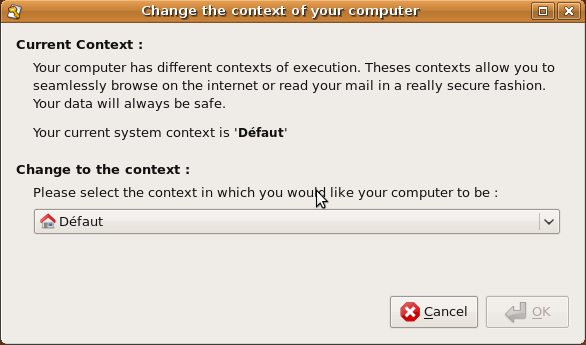
\includegraphics[width=11cm]{images/contextnotifydlg.png}
			\caption{Fenêtre de changement manuel de contexte}
			\label{context-notify change context}
		\end{figure}
		
		\begin{figure}[!h]
			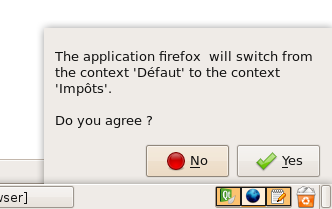
\includegraphics[width=7cm]{images/contextnotifypopup.png}
			\caption{Demande d'autorisation de transition}
			\label{context-notify autorisation}
		\end{figure}

	%Figure qui montre tout le userspace
	\begin{figure}[!h]
		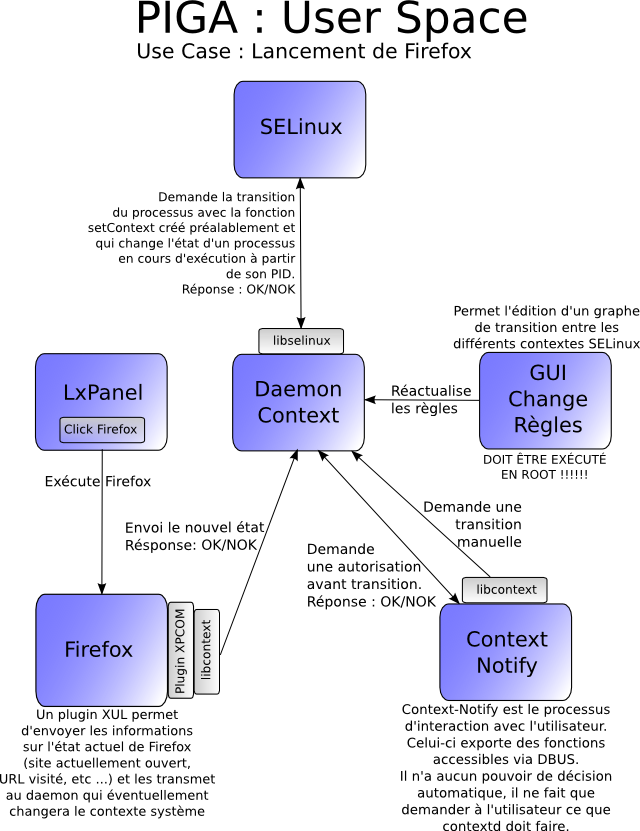
\includegraphics[width=17cm]{images/userspace.png}
		\caption{Schéma des interactions dans PIGA-SYSTRANS}
		\label{schema_piga_systrans}
	\end{figure}
		
\chapter{Les plugins}
	\label{PIGA_SYSTRANS plugins}
	
	\paragraph*{}
		Pour l'intégration de PIGA-SYSTRANS dans les applications, l'utilisation de plugins a semblé la meilleure option car elle est la plus pérenne/demande peu de temps à maintenir.
		
	\paragraph*{}
		Chaque plugin réalise deux tâches essentielles:
		\begin{itemize}
   			\item Transmettre l'état actuel du programme;
   			\item Changer dynamiquement l'affichage en fonction du contexte actuel et de ses droits;
   		\end{itemize}
	
	\section{Firefox}
		\paragraph*{}
			Le plugin Firefox réalise les deux tâches essentielles mais il se charge aussi de vider le cache lors d'un changement de contexte.
			
		\paragraph*{}
			Il est composé de deux parties:
			\begin{itemize}
   				\item Un plugin binaire XPCOM, écrit en C. Il permet d'établir le dialogue avec le daemon;
   				\item Un plugin Javascript. Il se charge de récupérer les événements utilisateur, de modifier l'interface graphique et de vider le cache lors des changements de contexte.
   			\end{itemize}
   			
   		\begin{figure}[!h]
			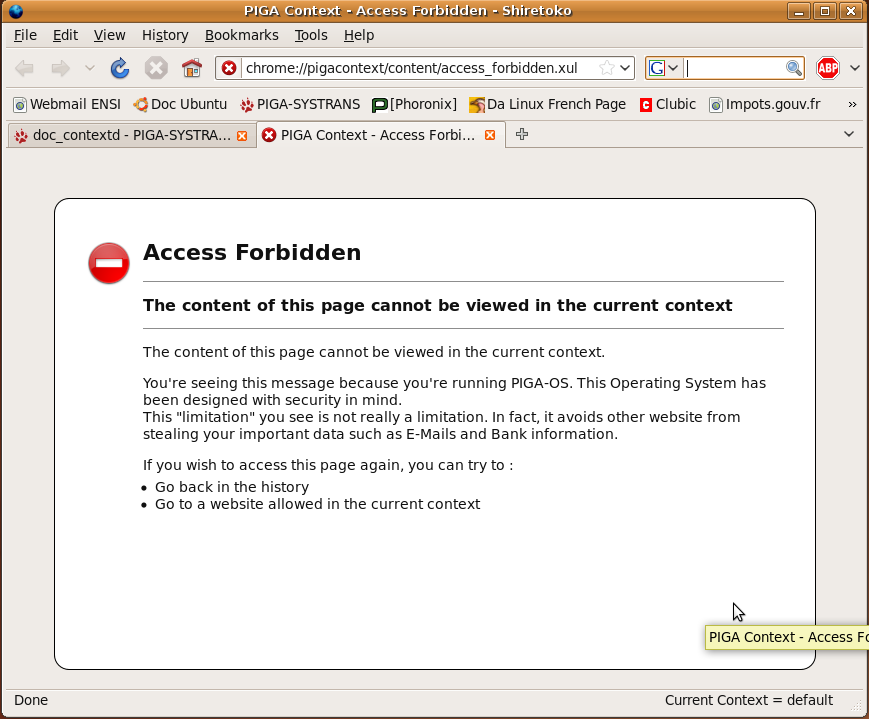
\includegraphics[width=13cm]{images/firefox.png}
			\caption{Exemple d'une modification faite à Firefox}
		\end{figure}
	
	\section{Claws-mail}
		\paragraph*{}
			Le plugin Claws-mail a été écrit en C/GTK. Cependant, contrairement à Firefox, il a nécessité des modifications dans le code de Claws-mail.
			
		\paragraph*{}
			En effet, Claws-mail n'avait aucun hook lors de l'ouverture d'un email et manquait aussi d'un système d'affichage d'erreur personnalisé à la place d'un email. Cela a été ma première tâche.
			
		\paragraph*{}
			Ces modifications ont été faites avec l'aval de l'équipe de Claws-mail. Pour ce faire, j'ai travaillé avec eux via IRC en leur expliquant premièrement ce que j'allais faire puis en leur soumettant des versions de test pour qu'ils puissent les pré-valider.\\
			Ce travail a été très intéressant et a été l'occasion de produire mon premier patch pour un programme autre que le mien. Je voudrais aussi saluer le professionnalisme de l'équipe, pourtant petite, qui montre bien que le logiciel libre n'est pas du travail d'amateur.
			
		\paragraph*{}
			Le patch final, qui fait environ 200 lignes, se trouve à l'adresse \emph{plugins/claws\-mail/mail\_pre\_open\_hook.patch}. Il sera proposé à la communauté pour approbation finale quand il aura été validé de notre coté.
			
		\begin{figure}[!h]
			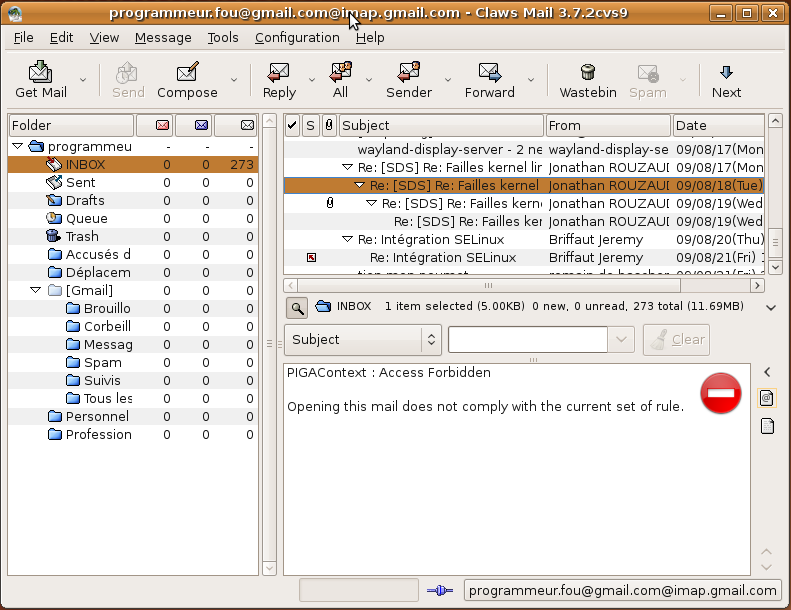
\includegraphics[width=13cm]{images/clawsmail.png}
			\caption{Exemple d'une modification faite à Claws-mail}
		\end{figure}
	
	\section{Open Office}
		\paragraph*{}
			Je n'ai malheureusement pas eu le temps d'aller plus loin que la recherche d'informations sur les plugins UNO.
			
		\paragraph*{}
			Ce plugin n'a donc pas pu être développé.
	
\chapter{Libcontext's Interface}
	\label{PIGA_SYSTRANS Libcontext Interface}
	{\tt \#include $<$string.h$>$}\par


Include dependency graph for libcontext.h:\nopagebreak
\begin{figure}[H]
\begin{center}
\leavevmode
\begin{figure}[!h]
	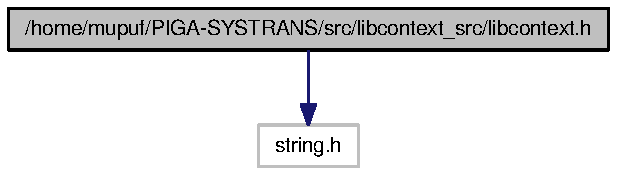
\includegraphics[width=166pt]{doxygen/libcontext_8h__incl}
	\caption{libcontext.h's dependency graph}
\end{figure}
\end{center}
\end{figure}


This graph shows which files directly or indirectly include this file:\nopagebreak
\begin{figure}[H]
\begin{center}
\leavevmode
\begin{figure}[!h]
	\includegraphics[width=357pt]{doxygen/libcontext_8h__dep__incl}
	\caption{libcontext.h is a dependency of ...}
\end{figure}
\end{center}
\end{figure}
\subsection*{Typedefs}
\begin{CompactItemize}
\item 
typedef void($\ast$ {\bf contextChangedCallbackSuccess} )(unsigned int id, {\bf context\_\-result} result)\label{libcontext_8h_5dda83b6631815ae03c1e487a549ba4a}

\begin{CompactList}\small\item\em id= \item\end{CompactList}\item 
typedef void($\ast$ \textbf{contextChangedCallbackError} )(unsigned int id, const char $\ast$error, const char $\ast$message)\label{libcontext_8h_5565e3ea8ade2cb600ae3b07aca2c281}

\item 
typedef void($\ast$ \textbf{contextChangedCallback} )(const char $\ast$previousContext, const char $\ast$nextContext, void $\ast$user\_\-data)\label{libcontext_8h_2fe3b642ce5c55f396c7889da7365fa3}

\end{CompactItemize}
\subsection*{Enumerations}
\begin{CompactItemize}
\item 
enum {\bf context\_\-bool} \{ {\bf CONTEXT\_\-FALSE} = 0, 
{\bf CONTEXT\_\-TRUE} = 1
 \}
\begin{CompactList}\small\item\em Define a boolean. \item\end{CompactList}\item 
enum {\bf context\_\-result} \{ {\bf CONTEXT\_\-ACCEPTED} = 0, 
{\bf CONTEXT\_\-REFUSED} = 1, 
{\bf CONTEXT\_\-ERROR} = 2
 \}
\begin{CompactList}\small\item\em Define context\_\-result. \item\end{CompactList}\end{CompactItemize}
\subsection*{Functions}
\begin{CompactItemize}
\item 
{\bf context\_\-bool} {\bf context\_\-is\_\-registered} ()
\begin{CompactList}\small\item\em Is your application already registered ? \item\end{CompactList}\item 
{\bf context\_\-bool} {\bf context\_\-register\_\-application} (const char $\ast$app\_\-name)
\begin{CompactList}\small\item\em Register your application onto the context Daemon. \item\end{CompactList}\item 
{\bf context\_\-result} {\bf context\_\-changed} (const char $\ast$param\_\-name,...)
\begin{CompactList}\small\item\em Send your internal context to the daemon. Should be called like this: context\_\-changed(var1\_\-name, var1\_\-data, var2\_\-name, var2\_\-data, ..., NULL, NULL);. \item\end{CompactList}\item 
unsigned int {\bf context\_\-changed\_\-async} ({\bf contextChangedCallbackSuccess} success\_\-cb, contextChangedCallbackError error\_\-cb, const char $\ast$param\_\-name,...)
\begin{CompactList}\small\item\em It the same than context\_\-changed but async, see \doxyref{context\_\-changed()}{p.}{libcontext_8h_efe26a27281f13bf1a919ca652c93f3c} for more details. \item\end{CompactList}\item 
{\bf context\_\-bool} {\bf context\_\-required\_\-context} (char $\ast$required\_\-context, size\_\-t maxlen, const char $\ast$param\_\-name,...)
\begin{CompactList}\small\item\em Checks what would be the system context if we had sent this state to the daemon. This is the same logic than \doxyref{context\_\-changed()}{p.}{libcontext_8h_efe26a27281f13bf1a919ca652c93f3c} with only some extra parameters. \item\end{CompactList}\item 
{\bf context\_\-bool} {\bf context\_\-current\_\-local\_\-context} (char $\ast$state\_\-buf, unsigned int max\_\-size)
\begin{CompactList}\small\item\em Get the local context of the currently registered process. \item\end{CompactList}\item 
{\bf context\_\-bool} {\bf context\_\-current\_\-global\_\-context} (char $\ast$state\_\-buf, unsigned int max\_\-size)
\begin{CompactList}\small\item\em Get the global context of the currently registered process. \item\end{CompactList}\item 
const char $\ast$ {\bf context\_\-getLastError} ()
\begin{CompactList}\small\item\em Returns the last error that happened. \item\end{CompactList}\item 
void {\bf context\_\-set\_\-context\_\-changed\_\-callback} (contextChangedCallback ccc, void $\ast$user\_\-data)\label{libcontext_8h_0e551d119c9f61cf4f77395a8c3d585a}

\begin{CompactList}\small\item\em Should not be used yet, it is not ready !! \item\end{CompactList}\end{CompactItemize}


\subsection*{Detailed Description}
\begin{Desc}
\item[Author:]Martin Peres (martin$<$dot$>$peres$<$At$>$ensi-bourges$<$dot$>$fr) \end{Desc}
\begin{Desc}
\item[Date:]27-08-2009 \end{Desc}


\subsection{Enumeration Type Documentation}
\index{libcontext.h@{libcontext.h}!context\_\-bool@{context\_\-bool}}
\index{context\_\-bool@{context\_\-bool}!libcontext.h@{libcontext.h}}
\subsubsection[{context\_\-bool}]{\setlength{\rightskip}{0pt plus 5cm}enum {\bf context\_\-bool}}\label{libcontext_8h_fcaa7d501c8b7b0694706fa156416a46}


Define a boolean. 

\begin{Desc}
\item[Enumerator: ]\par
\begin{description}
\index{CONTEXT\_\-FALSE@{CONTEXT\_\-FALSE}!libcontext.h@{libcontext.h}}\index{libcontext.h@{libcontext.h}!CONTEXT\_\-FALSE@{CONTEXT\_\-FALSE}}\item[{\em 
CONTEXT\_\-FALSE\label{libcontext_8h_fcaa7d501c8b7b0694706fa156416a46baf236655387c6cd1ffd7b3f7624443e}
}]FALSE. \index{CONTEXT\_\-TRUE@{CONTEXT\_\-TRUE}!libcontext.h@{libcontext.h}}\index{libcontext.h@{libcontext.h}!CONTEXT\_\-TRUE@{CONTEXT\_\-TRUE}}\item[{\em 
CONTEXT\_\-TRUE\label{libcontext_8h_fcaa7d501c8b7b0694706fa156416a467c0a09661e989aeab34b692fec0847a3}
}]TRUE. \end{description}
\end{Desc}

\index{libcontext.h@{libcontext.h}!context\_\-result@{context\_\-result}}
\index{context\_\-result@{context\_\-result}!libcontext.h@{libcontext.h}}
\subsubsection[{context\_\-result}]{\setlength{\rightskip}{0pt plus 5cm}enum {\bf context\_\-result}}\label{libcontext_8h_c420c905cf5447135932bd35cc019450}


Define context\_\-result. 

\begin{Desc}
\item[Enumerator: ]\par
\begin{description}
\index{CONTEXT\_\-ACCEPTED@{CONTEXT\_\-ACCEPTED}!libcontext.h@{libcontext.h}}\index{libcontext.h@{libcontext.h}!CONTEXT\_\-ACCEPTED@{CONTEXT\_\-ACCEPTED}}\item[{\em 
CONTEXT\_\-ACCEPTED\label{libcontext_8h_c420c905cf5447135932bd35cc0194504dba0c61d83b4e457e5fbe8affcf027d}
}]Accepted. \index{CONTEXT\_\-REFUSED@{CONTEXT\_\-REFUSED}!libcontext.h@{libcontext.h}}\index{libcontext.h@{libcontext.h}!CONTEXT\_\-REFUSED@{CONTEXT\_\-REFUSED}}\item[{\em 
CONTEXT\_\-REFUSED\label{libcontext_8h_c420c905cf5447135932bd35cc019450e56cab3063b05190d1e49f6e358b8ff1}
}]Refused. \index{CONTEXT\_\-ERROR@{CONTEXT\_\-ERROR}!libcontext.h@{libcontext.h}}\index{libcontext.h@{libcontext.h}!CONTEXT\_\-ERROR@{CONTEXT\_\-ERROR}}\item[{\em 
CONTEXT\_\-ERROR\label{libcontext_8h_c420c905cf5447135932bd35cc019450d4b4b5d5d1532329219cee4d8b4d33f7}
}]Error. \end{description}
\end{Desc}



\subsection{Function Documentation}
\index{libcontext.h@{libcontext.h}!context\_\-changed@{context\_\-changed}}
\index{context\_\-changed@{context\_\-changed}!libcontext.h@{libcontext.h}}
\subsubsection[{context\_\-changed}]{\setlength{\rightskip}{0pt plus 5cm}{\bf context\_\-result} context\_\-changed (const char $\ast$ {\em param\_\-name}, \/   {\em ...})}\label{libcontext_8h_efe26a27281f13bf1a919ca652c93f3c}


Send your internal context to the daemon. Should be called like this: context\_\-changed(var1\_\-name, var1\_\-data, var2\_\-name, var2\_\-data, ..., NULL, NULL);. 

\begin{Desc}
\item[Returns:]Returns CONTEXT\_\-ACCEPTED if the state is accepted by the daemon, CONTEXT\_\-REFUSED if the daemon refused it and CONTEXT\_\-ERROR if an error occured (see \doxyref{context\_\-getLastError()}{p.}{libcontext_8h_01f45cfc672e55f85cfc3ee462398e80}). If the daemon refused your internal state, you should go to another one that will be accepted (go back to the previous one or display an error message) !! \end{Desc}
\index{libcontext.h@{libcontext.h}!context\_\-changed\_\-async@{context\_\-changed\_\-async}}
\index{context\_\-changed\_\-async@{context\_\-changed\_\-async}!libcontext.h@{libcontext.h}}
\subsubsection[{context\_\-changed\_\-async}]{\setlength{\rightskip}{0pt plus 5cm}unsigned int context\_\-changed\_\-async ({\bf contextChangedCallbackSuccess} {\em success\_\-cb}, \/  contextChangedCallbackError {\em error\_\-cb}, \/  const char $\ast$ {\em param\_\-name}, \/   {\em ...})}\label{libcontext_8h_1d4c82efb9ac16f848b361f88caeddd1}


It the same than context\_\-changed but async, see \doxyref{context\_\-changed()}{p.}{libcontext_8h_efe26a27281f13bf1a919ca652c93f3c} for more details. 

\begin{Desc}
\item[Parameters:]
\begin{description}
\item[{\em success\_\-cb}]The callback to be called when the call succeded (check result) \item[{\em error\_\-cb}]The callback to call in case of an error. \end{description}
\end{Desc}
\begin{Desc}
\item[Returns:]Returns the ID of the call. This will also be put as a parameter in the callbacks so as you can match them. \end{Desc}
\index{libcontext.h@{libcontext.h}!context\_\-current\_\-global\_\-context@{context\_\-current\_\-global\_\-context}}
\index{context\_\-current\_\-global\_\-context@{context\_\-current\_\-global\_\-context}!libcontext.h@{libcontext.h}}
\subsubsection[{context\_\-current\_\-global\_\-context}]{\setlength{\rightskip}{0pt plus 5cm}{\bf context\_\-bool} context\_\-current\_\-global\_\-context (char $\ast$ {\em state\_\-buf}, \/  unsigned int {\em max\_\-size})}\label{libcontext_8h_853de71f6d9dd38312193f560dbb2d0d}


Get the global context of the currently registered process. 

\begin{Desc}
\item[Parameters:]
\begin{description}
\item[{\em state\_\-buf}]out: The buffer that will receive the name of the context. \item[{\em max\_\-size}]in: The size of the buffer \end{description}
\end{Desc}
\begin{Desc}
\item[Returns:]Returns CONTEXT\_\-TRUE if the context has been retrieved, CONTEXT\_\-FALSE otherwise \end{Desc}
\index{libcontext.h@{libcontext.h}!context\_\-current\_\-local\_\-context@{context\_\-current\_\-local\_\-context}}
\index{context\_\-current\_\-local\_\-context@{context\_\-current\_\-local\_\-context}!libcontext.h@{libcontext.h}}
\subsubsection[{context\_\-current\_\-local\_\-context}]{\setlength{\rightskip}{0pt plus 5cm}{\bf context\_\-bool} context\_\-current\_\-local\_\-context (char $\ast$ {\em state\_\-buf}, \/  unsigned int {\em max\_\-size})}\label{libcontext_8h_f1335ac681f3b57eb53c1834148e7aa5}


Get the local context of the currently registered process. 

\begin{Desc}
\item[Parameters:]
\begin{description}
\item[{\em state\_\-buf}]out: The buffer that will receive the name of the context. \item[{\em max\_\-size}]in: The size of the buffer \end{description}
\end{Desc}
\begin{Desc}
\item[Returns:]Returns CONTEXT\_\-TRUE if the context has been retrieved, CONTEXT\_\-FALSE otherwise \end{Desc}
\index{libcontext.h@{libcontext.h}!context\_\-getLastError@{context\_\-getLastError}}
\index{context\_\-getLastError@{context\_\-getLastError}!libcontext.h@{libcontext.h}}
\subsubsection[{context\_\-getLastError}]{\setlength{\rightskip}{0pt plus 5cm}const char$\ast$ context\_\-getLastError ()}\label{libcontext_8h_01f45cfc672e55f85cfc3ee462398e80}


Returns the last error that happened. 

\begin{Desc}
\item[Returns:]Returns the last error that happened. \end{Desc}
\index{libcontext.h@{libcontext.h}!context\_\-is\_\-registered@{context\_\-is\_\-registered}}
\index{context\_\-is\_\-registered@{context\_\-is\_\-registered}!libcontext.h@{libcontext.h}}
\subsubsection[{context\_\-is\_\-registered}]{\setlength{\rightskip}{0pt plus 5cm}{\bf context\_\-bool} context\_\-is\_\-registered ()}\label{libcontext_8h_78e7738e37581c0187e8a482747bded2}


Is your application already registered ? 

\begin{Desc}
\item[Returns:]Returns CONTEXT\_\-TRUE if the application is registered \end{Desc}
\index{libcontext.h@{libcontext.h}!context\_\-register\_\-application@{context\_\-register\_\-application}}
\index{context\_\-register\_\-application@{context\_\-register\_\-application}!libcontext.h@{libcontext.h}}
\subsubsection[{context\_\-register\_\-application}]{\setlength{\rightskip}{0pt plus 5cm}{\bf context\_\-bool} context\_\-register\_\-application (const char $\ast$ {\em app\_\-name})}\label{libcontext_8h_ad1b2d46c9febbc5d3ea0443a6680e22}


Register your application onto the context Daemon. 

\begin{Desc}
\item[Parameters:]
\begin{description}
\item[{\em app\_\-name}]The name of your application. \end{description}
\end{Desc}
\begin{Desc}
\item[Returns:]Returns CONTEXT\_\-TRUE if the application has been successfuly registered \end{Desc}
\index{libcontext.h@{libcontext.h}!context\_\-required\_\-context@{context\_\-required\_\-context}}
\index{context\_\-required\_\-context@{context\_\-required\_\-context}!libcontext.h@{libcontext.h}}
\subsubsection[{context\_\-required\_\-context}]{\setlength{\rightskip}{0pt plus 5cm}{\bf context\_\-bool} context\_\-required\_\-context (char $\ast$ {\em required\_\-context}, \/  size\_\-t {\em maxlen}, \/  const char $\ast$ {\em param\_\-name}, \/   {\em ...})}\label{libcontext_8h_fc46d75cc9a90535237149b2646e24e0}


Checks what would be the system context if we had sent this state to the daemon. This is the same logic than \doxyref{context\_\-changed()}{p.}{libcontext_8h_efe26a27281f13bf1a919ca652c93f3c} with only some extra parameters. 

\begin{Desc}
\item[Parameters:]
\begin{description}
\item[\mbox{$\rightarrow$} {\em required\_\-context}]The buffer where the name of the context will be put. \item[{\em maxlen}]The size of the buffer required\_\-context minus one. \end{description}
\end{Desc}
\begin{Desc}
\item[Returns:]Returns CONTEXT\_\-TRUE if everything went fine and if the context is stored in required\_\-context. CONTEXT\_\-FALSE otherwise. \end{Desc}

	
\chapter{La documentation disponible sur le wiki du Trac du projet (anglais)}
	\label{PIGA_SYSTRANS TRAC}
	
	
\end{document}